\documentclass{officialexam} 
\usepackage{circuitikz}
\everymath{\color{blue}}
\usepackage{graphicx}
\graphicspath{ {./images/} }
\begin{document}
	\begin{center}
		\sffamily\color{blue}
		\huge ជំពូក១~\color{red}ផលរង្វិលនៃកម្លាំង
	\end{center}
	\borderline{\fbox{លំហាត់ៈ បង្គុំ និងបំបែកកម្លាំង}}
	\begin{enumerate}[m]
		\item បន្ទាត់ស្មើសាច់មួយមានប្រវែង $50cm$ ចុងសងខាងនៃបន្ទាត់រងនូវកម្លាំងពីរស្របគ្នា និងមានទិសដៅដូចគ្នា។ កម្លាំងទីមួយស្មើនឹង $600N$ និងកម្លាំងទីពីរស្មើនឹង $400N$។ កំណត់កម្លាំងផ្គួបនៃកម្លាំងទាំងពីរ។
		\item បន្ទាត់ស្មើសាច់មួយមានប្រវែង $100cm$ រងនូវកម្លាំងបីស្របគ្នា និងមានទិសដៅដូចគ្នា។ ចុងខាងស្តាំងរងនូវកម្លាំងមួយស្មើនឹង $20N$\\ ឯចុងខាងឆ្វេងរងនូវកម្លាំងមួយស្មើ $90N$ និងកណ្តាលរងនូវកម្លាំង $30N$។ គណនាកម្លាំងផ្គួបនៃកម្លាំងទាំងបី។
		\item របារមួយទ្រដោយទម្រ $A$ និង $B$ ដែលមានចម្ងាយពីគ្នា $5m$។ របារទ្រទម្ងន់ស្មើនឹង $40000N$ ត្រង់ចំណុចចាប់មួយដែលមានចម្ងាយពីចំណុច $A$ ប្រវែង $2.6m$។ កំណត់កម្លាំងដែលមានអំពើលើទម្រ $A$ និងទម្រ $B$(មិនគិតទម្ងន់ទម្ររបារ)។
		\item កម្លាំងពីរ $\overrightarrow{F}_{1}$ និង $\overrightarrow{F}_{2}$ មានទិសកែងគ្នា មានអាំងតង់សុីតេរៀងគ្នា $4N$ និង $7N$ មានចំណុចចាប់រួម $O$។\\
		គូសវុិចទ័រតាងកម្លាំងផ្គួបនៃកម្លាំងទាំងពីរ និងរកអាំងតង់សុីតេកម្លាំងផ្គួបនេះដោយប្រើមាត្រដ្ឋាន $1cm=1N$។
		\item កម្លាំងមួយ $50N$ មានទិសដៅបង្កើតបានមុំ $45^\circ$ តាមទិសដេក។ រកកម្លាំងផ្គុំឈរ និងកម្លាំងផ្គុំដេករបស់វា។ 
	\end{enumerate}
	\borderline{\fbox{លំហាត់ៈ ម៉ូម៉ង់នៃកម្លាំង}}
	\begin{enumerate}[m]
		\item ដូចម្តេចដែលហៅថាម៉ូម៉ង់នៃកម្លាំង?
		\item ចូរសរសេររូបមន្តម៉ូម៉ង់នៃកម្លាំង និងបញ្ជាក់ខ្នាតនៃទំហំទាំងអស់ក្នុងរូបមន្ត។
		\item ហេតុអ្វីបានជាគេយកដៃរុញទ្វារក្បែរត្រចៀករបស់វាពិបាកបើកជាងយកដៃរុញត្រង់គែមទ្វារ ឬត្រង់សោទ្វារ?
		\item គេបញ្ជេគកម្លាំង $10N$ កែងនឹងសោមួយដែលមានប្រវែង $0.2m$។ គណនាម៉ូម៉ង់នៃកម្លាំងបង្វិលខ្ខៅក្នុងករណីៈ
		\begin{enumerate}[k]
			\item ចំណុចចាប់នៃកម្លាំងស្ថិតត្រង់ចំណុចកណ្តាលនៃដងសោ។
			\item ចំណុចចាប់នៃកម្លាំងស្ថិតត្រង់ចំណុចចុងដងសោ។
		\end{enumerate}
		\item គណនាម៉ូម៉ង់កម្លាំងដូចរូបដែលចំណុច $O$ ជាអ័ក្សរង្វិលៈ
		\begin{multicols}{4}
			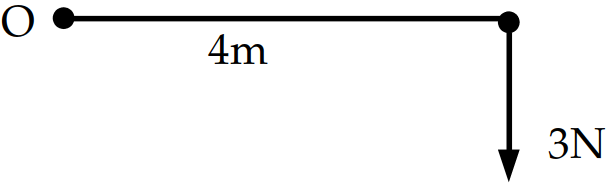
\includegraphics[scale=0.25]{01}
			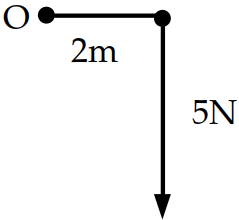
\includegraphics[scale=0.3]{02}
			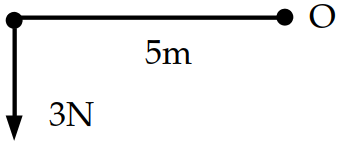
\includegraphics[scale=0.3]{03}
			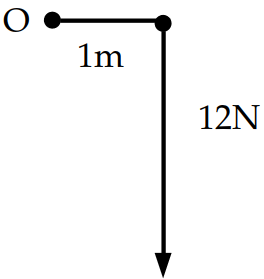
\includegraphics[scale=0.3]{04}
		\end{multicols}
		\item មនុស្សម្នាក់មានទម្ងន់ $600N$ អង្គុយនៅលើចុងម្ខាងនៃដងថ្លឹងមួយស្ថិតចម្ងាយ $1.5m$ ពីអ័ក្សរង្វិល។ ដើម្បីឲ្យដងថ្លឹងមានលំនឹងតាមទិសដេក តើមនុស្សម្នាក់ទៀតដែលត្រូវអង្គុយនៅចុងម្ខាងទៀតនៃដងថ្លឹងស្ថិតចម្ងាយ $2m$ ពីអ័ក្សរង្វិលមានទម្ងន់ប៉ុន្មាន?
		\item គេព្យួរអង្គធាតុពីរមានទម្ងន់ $F_1=400N$ និង $F_2=100N$ ទៅនឹងចុងសងខាងនៃរបារស្មើសាច់មួយទម្ងន់ $F_{3}=100N$ ប្រវែង $d=40cm$។ តើគេត្រូវដាក់កំណល់ត្រង់កន្លែងណានៃរបារដើម្បីឲ្យវាមានលំនឹង?
	\end{enumerate}\newpage
	\borderline{\fbox{លំហាតៈ ទីប្រជុំទម្ងន់}}
	\begin{enumerate}[m]
		\item ដូចម្តេចដែលហៅថាទីប្រជុំទម្ងន់? តើវត្ថុ ឬអង្គធាតុមួយមានទីប្រជុំទម្ងន់ប៉ុន្មាន?
		\item តើគេប្រើវិធីអ្វីដើម្បីរកទីប្រជុំទម្ងន់នៃអង្គធាតុរឹងស្មើសាច់មួយមិនរាងធរណីមាត្រងាយ?
		\item តើអ្នកអាចរកទីប្រជុំទម្ងន់នៃបន្ទាត់ក្រិតរបស់អ្នកដោយមិនចាំបាច់ប្រើវិធីព្យួរបានដែរ ឬទេ?
		\item ចូរកាត់ក្រដាសរឹងជារូបផែនទីប្រទេសកម្ពុជាហើយរកទីប្រជុំទម្ងន់របស់វា។ តើទីប្រជុំទម្ងន់នៃប្រទេសកម្ពុជាស្ថិតនៅក្នុងខេត្តណា?
		\item ហេតុអ្វីបានជាយើងមិនត្រូវផ្ទុកឥវ៉ាន់ធ្ងន់ៗលើដំបូលរទេះ ឬដំបូលរថយន្តឲ្យខ្ពស់នៅពេលកំពុងបើកបរ? ចូរពន្យល់។
	\end{enumerate}
	\borderline{\fbox{សំណួរ និងលំហាត់ជំពូក១}}
	\begin{enumerate}[I]
		\item {\color{khtug}\sffamily ចូរគូសសញ្ញា \tick ~ក្នុងប្រអប់មុខចម្លើយត្រឹមត្រវដែលមានតែមួយគត់ៈ}
		\begin{enumerate}[m]
			\item ម៉ូម៉ង់កម្លាំងមួយជាទំហំកំណត់ដោយៈ
			\begin{multicols}{2}
				\begin{enumerate}[bk]
					\item ផលចែករវាងកម្លាំង និងប្រវែងដៃឃ្នាស់។
					\item ផលគុណរវាងកម្លាំង និងប្រវែងដៃឃ្នាស់។
					\item ផលបូករវាងកម្លាំង និងប្រវែងដៃឃ្នាស់។
					\item ផលដករវាងកម្លាំង និងប្រវែងដៃឃ្នាស់។
				\end{enumerate}
			\end{multicols}
			\item អង្គធាតុរឹងមួយដែលអាចចល័តជុំវុិញអ័ក្សមួយ មានលំនឹងកាលណាៈ
			\begin{enumerate}[bk]
				\item ផលបូកម៉ូម៉ង់នៃកម្លាំងមានអំពើលើអង្គធាតុនោះស្មើសូន្យ។
				\item ផលដកម៉ូម៉ង់នៃកម្លាំងមានអំពើលើអង្គធាតុនោះស្មើសូន្យ។
				\item ផលចែកម៉ូម៉ង់នៃកម្លាំងមានអំពើលើអង្គធាតុនោះស្មើសូន្យ។
				\item ផលគុណម៉ូម៉ង់នៃកម្លាំងមានអំពើលើអង្គធាតុនោះស្មើសូន្យ។
			\end{enumerate}
			\item ទីប្រជុំទម្ងន់របស់អង្គធាតុមួយគឺៈ
			\begin{enumerate}[bk]
				\item ជាចំណុចកណ្តាលនៃអង្គធាតុនោះ។
				\item ជាចំណុចមួមយដែលធ្វើឲ្យអង្គធាតុនោះមានលំនឹង។
				\item ជាចំណុចមួយដែលទម្ងន់នៃអង្គធាតុទាំងមូលហាក់បីដូចជាមកផ្តុំគ្នាត្រង់ចំណុចនោះ។
				\item ជាចំណុចមួយស្ថិតនៅលើអង្កត់ទ្រូងរបស់អង្គធាតុ។
			\end{enumerate}
			\item ក្នុងបណ្តារូបខាងក្រោម តើរូបមួយណាដែលបង្ហាញពីលំនឹងគ្រប់ទិសទី?
			\begin{multicols}{4}
				\begin{enumerate}[bk]
					\item 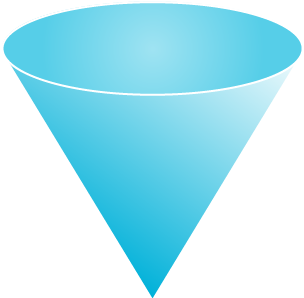
\includegraphics[scale=1]{05}
					\item 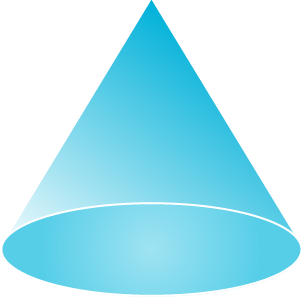
\includegraphics[scale=1]{06}
					\item 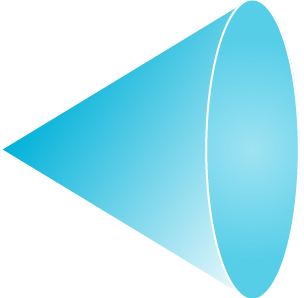
\includegraphics[scale=1]{07}
					\item 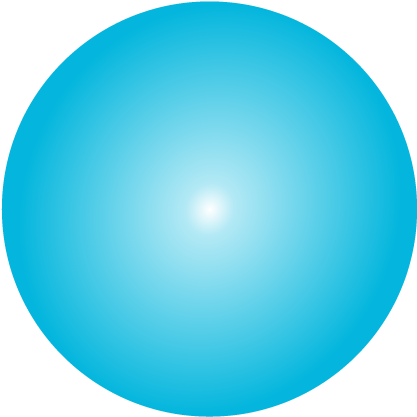
\includegraphics[scale=0.7]{08}
				\end{enumerate}
			\end{multicols}
		\end{enumerate}
		\item {\color{khtug}\sffamily ចូរបំពេញល្បះខាងក្រោមឲ្យបានត្រឹមត្រូវៈ}
		\begin{enumerate}[m]
			\item ចម្ងាយរវាងអ័ក្សរង្វិលទៅខ្សែសកម្មនៃកម្លាំងហៅថា \dotfill។
			\item ម៉ូម៉ង់នៃកម្លាំងដែលធ្វើឲ្យអង្គធាតុមួយវិលតាមទិសដៅរង្វិលនៃទ្រនិចនាឡិកាហៅថា\dotfill។
			\item ម៉ូម៉ង់នៃកម្លាំងដែលធ្វើឲ្យអង្គធាតុមួយវិលតាមទិសដៅបញ្រ្ចាសនឹងរង្វិលនៃទ្រនិចនាឡិកាហៅថា\dotfill។
			\item អង្គធាតុរឹងមួយស្ថិតនៅលើប្លង់ដេក កាលណាខ្សែឈរនៃទីប្រជុំទម្ងន់កាត់តាមចំណុចមួយស្ថិតក្នុងប្លង់បាតទម្រកាន់តែក្បែរផ្ចិតទម្រ គេថាអង្គធាតុនោះមានលំនឹង\dotfill។
			\item អង្គធាតុរឹងមួយស្ថិតនៅលើប្លង់ដេក កាលណាទីប្រជុំទម្ងន់របស់វាស្ថិតនៅកាន់តែខ្ពស់ និងខ្សែឈរនៃទីប្រជុំទម្ងន់កាត់តាមចំណុចមួយស្ថិតកាន់តែក្បែរបាតទម្រ ឬក្រៅបាតទម្រ គេថាអង្គធាតុនោះមានលំនឹង\dotfill។
		\end{enumerate}
		\item {\color{khtug}\sffamily លំហាត់}
		\begin{enumerate}[m]
			\item ទ្វារមួយត្រូវការម៉ូម៉ង់អប្បបរមា $32.5N\cdot m$ ដើម្បីបិទបើក។ តើគេត្រូវដាក់ដៃទ្វារនៅចម្ងាយប៉ុន្មានពីត្រចៀក បើគេដឹងថាដើម្បីបិទ ឬបើកគេត្រូវការបញ្ចេញកម្លាំងមិនលើពី $50N$?
			\item ក្នុងចំណោមរូបខាងក្រោម តើមួយណាមានម៉ូម៉ង់កម្លាំងធំជាងគេ? ម៉ូម៉ង់កម្លាំងតូចជាងគេ? មានម៉ូម៉ង់កម្លាំងស្មើគ្នា?
			\begin{multicols}{2}
				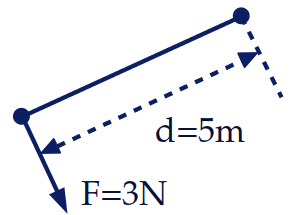
\includegraphics[scale=0.4]{09}
				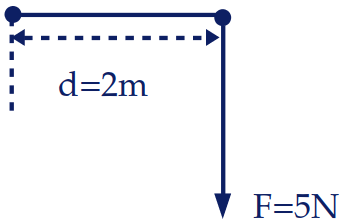
\includegraphics[scale=0.4]{10}
				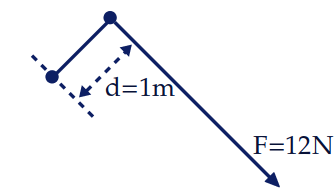
\includegraphics[scale=0.4]{11}
				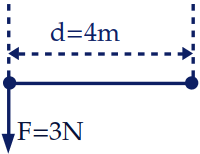
\includegraphics[scale=0.4]{12}
			\end{multicols}
		\end{enumerate}
	\begin{center}
		\sffamily\color{blue}
		សូមអានប្រធានលំហាត់ឲ្យបានច្បាស់មុនធ្វើលំហាត់!
	\end{center}
	\end{enumerate}
	\borderline{ដំណោះស្រាយ}\\
	{\color{white}.}\dotfill
	\\
	{\color{white}.}\dotfill\\
	{\color{white}.}\dotfill\\
	{\color{white}.}\dotfill
	\\
	{\color{white}.}\dotfill\\
	{\color{white}.}\dotfill\\
	{\color{white}.}\dotfill
	\\
	{\color{white}.}\dotfill\\
	{\color{white}.}\dotfill\\
	{\color{white}.}\dotfill
	\\
	{\color{white}.}\dotfill\\
	{\color{white}.}\dotfill\\
	{\color{white}.}\dotfill
	\\
	{\color{white}.}\dotfill\\
	{\color{white}.}\dotfill\\
	{\color{white}.}\dotfill
	\\
	{\color{white}.}\dotfill\\
	{\color{white}.}\dotfill\\
	{\color{white}.}\dotfill
	\\
	{\color{white}.}\dotfill\\
	{\color{white}.}\dotfill
	\begin{center}
		\sffamily\color{blue}
		សូមសំណាងល្អ!
	\end{center}\newpage
\begin{center}
	\sffamily\color{blue}
	\huge ជំពូក២~\color{red}ម៉ាសុីនងាយ
\end{center}
\borderline{\fbox{លំហាត់ៈ ឃ្នាស់}}
\begin{enumerate}[m]
	\item ដូចម្តេចដែលហៅថាឃ្នាស់? តើផ្នែកសំខាន់ៗនៃឃ្នាស់មានអ្វីខ្លះ?
	\item គេចែកឃ្នាស់ជាប៉ុន្មានប្រភេទ? អ្វីខ្លះ?
	\item ដូចម្តេចដែលហៅថាឃ្នាស់ទម្រកណ្តាល? ឃ្នាស់ទំនប់កណ្តាល? ឃ្នាស់ចលករកណ្តាល?
	\item ចូរឲ្យឧបករណ៍ដែលប្រើប្រាស់ឃ្នាស់ទម្រកណ្តាល ឃ្នាស់ទំនប់កណ្តាល និងឃ្នាស់ចលករកណ្តាល។
	\item ដូចម្តេចដែលហៅថាផលមេកានិចនៃឃ្នាស់?
	\item គេប្រើរបារដែកមួយមានប្រវែង $1.2m$ ធ្វើជាឃ្នាស់ដើម្បីគាស់បន្ទុកមួយមានម៉ាស $60kg$។ ចំណុចទម្រនៃឃ្នាស់ស្ថិតនៅចម្ងាយ $30cm$ ពីបន្ទុក។ គណនាផលមេកានិចនៃឃ្នាស់ និងគណនាកម្លាំងចលករ គេឲ្យៈ $g=10m/s^{2}$។
	\item បន្ទាត់មួយមានប្រវែង $50cm$ ចល័តជុំវិញអ័ក្សដេកមួយកាត់ទីប្រជុំទម្ងន់របស់វាដែលស្ថិតនៅចំកណ្តាលបន្ទាត់។ គេព្យួរទម្ងន់ $3N$ នៅចុងម្ខាងនៃបន្ទាត់នោះ។ តើគេព្យួរទម្ងន់ប៉ុន្មានញ៉ូតុននៅផ្នែកម្ខាងទៀតនៃអ័ក្សត្រង់ចំណុចមួយស្ថិតចម្ងាយ $20cm$ ពីអ័ក្សនោះ ដើម្បីរក្សាបន្ទាត់ឲ្យមានលំនឹងតាមអ័ក្សដេក?
	\item បន្ទុកមួយមានទម្ងន់ $40N$ នៅលើដងថ្លឹងដែលស្ថិតនៅចម្ងាយ $0.3m$ ពីទម្រ។ តើគេត្រូវដាក់បន្ទុកមួយទៀតដែលមានទម្ងន់ $60N$ នៅចម្ងាយប៉ុន្មានពីចំណុចទម្រនៅផ្នែកម្ខាងទៀត ដើម្បីឲ្យដងថ្លឹងមានលំនឹងតាមទិសដេក?
	\item ដងថ្លឹងមួយមានប្រវែង $30cm$។ នៅចុងសងខាងរបស់វាគេផ្ទុកទម្ងន់ $40N$ និង $80N$។ តើទីតាំងនៃចំណុចទម្រត្រូវស្ថិតនៅត្រង់ចំណុចណាដើម្បីឲ្យដងថ្លឹងមានលំនឹងតាមទិសដេក?
	\item \begin{multicols}{2}
		រូបស្តាំដៃ បង្ហាញពីបន្ទាត់ស្មើសាច់ព្យួរនឹងខ្សែមួយត្រង់ចំណុចកណ្តាល។ បន្ទាត់នេះថ្ពក់អង្គធាតុពីរហើយមានលំនឹងតាមទិសដេក។ តើអង្គធាតុ $A$ មានទម្ងន់ប៉ុន្មាន?
		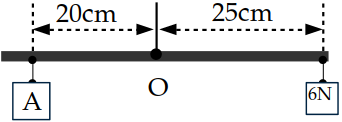
\includegraphics[scale=0.7]{13}
	\end{multicols}
	\item គេលើកអង្គធាតុមួយមានទម្ងន់ $60N$ ដោយប្រើឃ្នាស់ដូចរូបខាងក្រោម។ គណនាផលមេកានិច និងកម្លាំងចលករដែលមានអំពើលើឃ្នាស់ដើម្បីលើកអង្គធាតុនោះក្នុងករណីខាងក្រោមៈ\\
	\begin{center}
		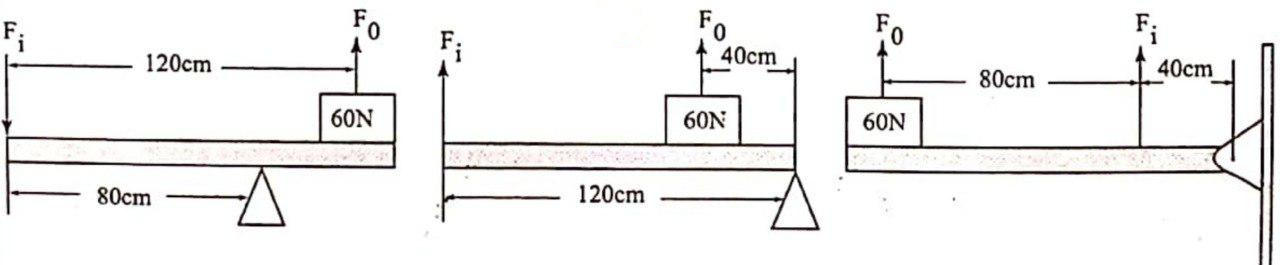
\includegraphics[scale=0.4]{14}
	\end{center}
\begin{center}
	\sffamily\color{blue}
	សូមអានប្រធានលំហាត់ឲ្យបានច្បាស់មុនធ្វើលំហាត់!
\end{center}
\end{enumerate}\newpage
\borderline{\fbox{លំហាត់ៈ ប្លង់ទេរ}}
\begin{enumerate}[m]
	\item ដូចម្តេចដែលហៅថាប្លង់ទេរ?
	\item ហេតុអ្វីបានទេគេចូលចិត្តប្រើប្លង់ទេដើម្បីរុញ ឬប្រមៀលធុងសាំងឡើងលើរថយន្ត?
	\item តើជណ្តើរឡើងផ្ទះរបស់អ្នកអាចចាត់ទុកជាប្លង់ទេដែរ ឬទេ?
	\item ក្នុងការលើកវត្ដុធ្ងន់ៗឡើងរថយន្ត តើគេជ្រើសរើសប្រវែងប្លង់ទេរដូចម្តេចទើបចំណេញកម្លាំងចលករបានច្រើន?
	\item រកផលមេកានិចនៃប្លង់ទេរខាងក្រោម។\\
	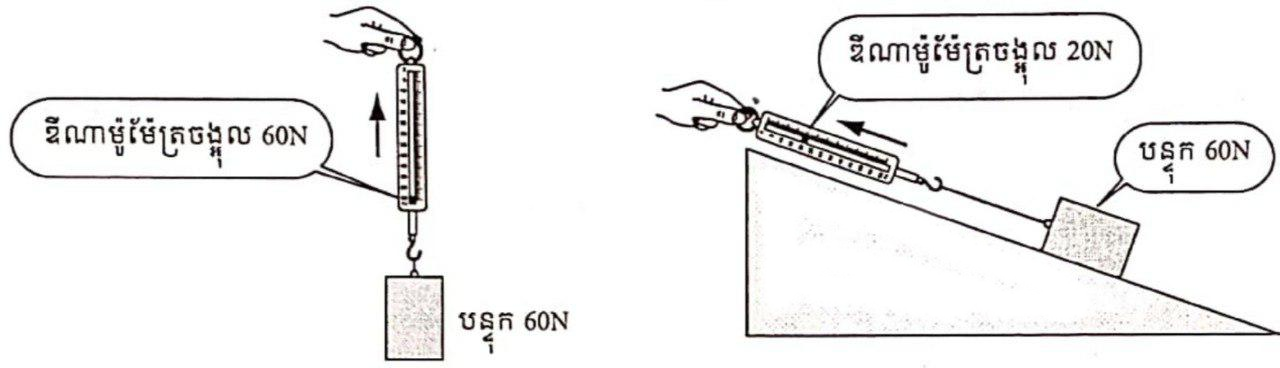
\includegraphics[scale=0.3]{15}
	\item ដើម្បីដាកធុងសាំងទម្ងន់ $1380N$ ចេញពីរថយន្ត កម្មករម្នាក់ប្រើប្លង់ទេរដែលមានប្រវែងវែងស្មើនឹង $6$ ដងនៃកម្ពស់។\\
	គណនាអាំងតង់សុីតេកម្លាំងដែលកម្មករនោះត្រូវបញ្ចេញដើម្បីទប់ធុងសាំងមិនឲ្យរមៀលធ្លាក់ចុះមកដី(មិនគិតកម្លាំងកកិត)។
	\item ផ្លូវចំណោតមួយមានប្រវែង $20m$ និងកម្ពស់ $4m$។ គណនាកម្មន្តដែលត្រូវបំពេញដើម្បីទាញវត្ថុមួយទម្ងន់ $150N$ ឲ្យដល់កំពូលចំណោត។ គណនាកម្លាំងដែលត្រូវផ្តល់ដើម្បីបំពេញកម្មន្តនេះ(មិនគិតកម្លាំងកកិត)។
\end{enumerate}
\borderline{\fbox{លំហាត់ៈ កង់យោង និងស្ពឺ}}
\begin{enumerate}[m]
	\item កង់ខ្លះមានលីបច្រើនជាន់ដែលអាចឲ្យអ្នកជិះប្តូរច្រវ៉ាក់ពីធំទៅតូច ឬពីតូចទៅធំបាន។ បើច្រវ៉ាក់ព័ទ្ធលើលីបធំ តើអ្នកធាក់ធូរ ឬតឹង? បើច្រវ៉ាក់ព័ទ្ធលើលីបតូចវិញ តើកម្លាំងធាក់ទៅជាយ៉ាងណា? បើតាមគោលការណ៍ម៉ូម៉ង់នៃកម្លាំងករណីប្រើលីបធំតើអ្នកចំណេញអ្វី និងខាតអ្វី? ហើយក្នុងករណីប្រើលីបតូច តើចំណេញអ្វី និងខាតអ្វី?
	\item ចូរធ្វើការវិភាគកម្លាំងចលករ និងកម្លាំងទប់នៃរហាត់ទឹក។ តើរហាត់ទឹកដែលមានកាំធំគេចំណេញអ្វី? ឯរហាត់ទឹកដែលមានកាំតូច តើគេចំណេញអ្វីដែរ? តើរហាត់ទឹកណាវិលលឿនជាងរហាត់ណា?
	\item ថាសឈ្នាន់កង់មួយមានធ្មេញ $42$ និងលីបមានធ្មេញ $14$។ បើគេធាក់ឈ្នាន់កង់បានបីជុំ តើលីបវិលបានប៉ុន្មានជុំ?
	\item ថាស់ឈ្នាន់កង់មួយមានធ្មេញ $51$ និងលីបមាន $17$។ គណនាផលមេកានិចនៃស្ពឺ។
	\item គេមានស្ពឺ $A,~B$ និង $C$ ដូចរូប។
	\begin{multicols}{2}
		\begin{enumerate}[k]
			\item ចូរគូសព្រួញបញ្ជាក់ពីទិសដៅរង្វិលនៃស្ពឺ $B$ និងស្ពឺ $C$ កាលណាស្ពឺ $A$ វិលតាមទិសដៅដូចរូប។
			\item គណនាចំនួនជុំក្នុងមួយវិនាទីនៃស្ពឺ $B$ និងស្ពឺ $C$ បើស្ពឺ $A$ វិលបាន $30\text{ជុំ}/s$។
		\end{enumerate}
		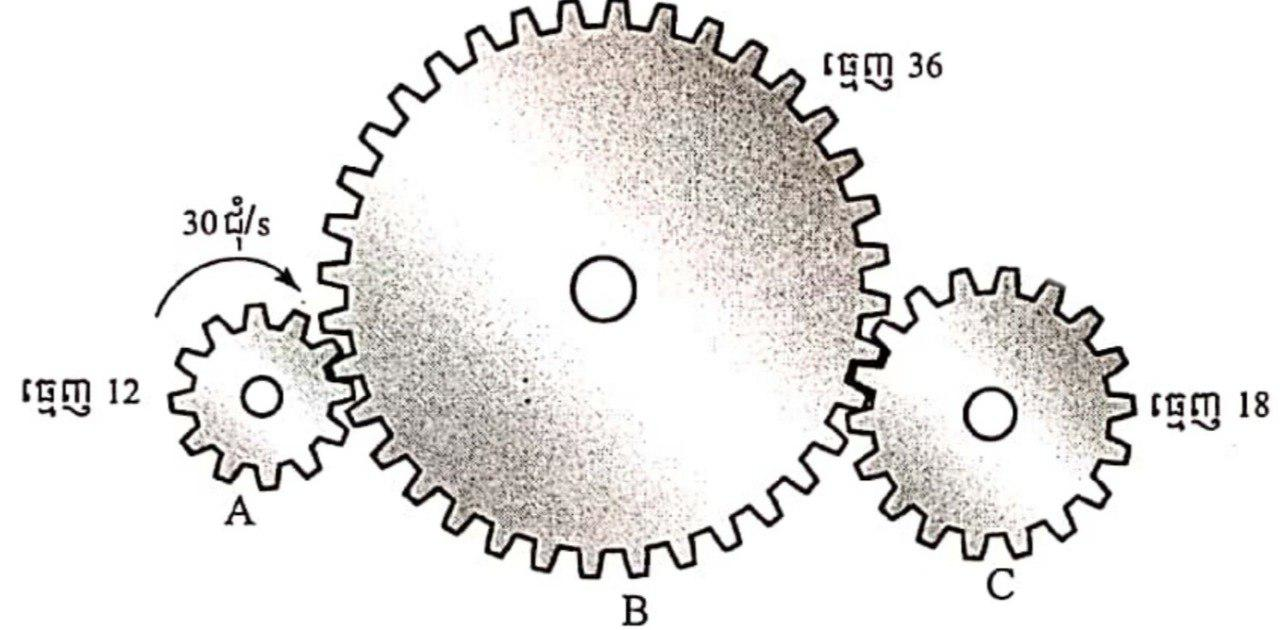
\includegraphics[scale=0.2]{16}
	\end{multicols}
	\item ជាងមកាត់ដេរម្នាក់បញ្ចេញកម្លាំង $200N$ ដើម្បីបង្វិលកង់យោងនៃឈ្នាន់ម៉ាសុីនដេរមួយដែលមានកាំ $30cm$។ ឯកង់យោងនៅត្រង់ក្បាលម៉ាសុីនមានកាំ $10cm$។
	\begin{enumerate}[k]
		\item គណនាកម្លាំងទប់របស់ក្បាលម៉ាសុីនដេរ(គេមិនគិតកកិតរវាងកង់យោង និងខ្សែពាន)។
		\item គណនាផលមេកានិចនៃកង់យោង។
		\item គណនាម៉ូម៉ង់កម្លាំងនៃកង់ចលករ និងម៉ូម៉ង់កម្លាំងនៃកង់ទប់។
	\end{enumerate}
\end{enumerate}
\borderline{\fbox{លំហាត់ៈ រ៉ក និងត្រឺយ}}
\begin{enumerate}[m]
	\item ដូចម្តេចដែលហៅថារ៉ក? តើរ៉កនឹង និងរ៉កចល័តខុសគ្នាដូចម្តេច?
	\item ដូចម្តេចដែលហៅថាត្រឺយ?
	\item តើផលមេកានិចនៃប្រព័ន្ធរ៉កនឹងមួយស្មើប៉ុន្មាន? តើផលមេកានិចនៃរ៉កចល័តមួយស្មើប៉ុន្មាន?
	\item តើផលមេកានិចនៃប្រព័ន្ធរ៉កមួយដែលផ្គុំរ៉កនឹងពីរ និងរ៉កចល័តមួយស្មើនឹងប៉ុន្មាន?
	\item គេប្រើរ៉កនឹងមួយលើកវត្ថុដែលមានម៉ាស $85kg$។ តើគេអាចលើកវត្ថុនោះបានដែរឬទេ បើគេបញ្ចេញកម្លាំងតែ $750N$?
	\item គេព្យួរវត្ថុមួយមានម៉ាស $59kg$ ទៅនឹងរ៉កចល័តមួយ។ គណនាអាំងតង់សុីតេកម្លាំងដែលមានអំពើទៅលើទំពក់ និងអាំងតង់សុីតេកម្លាំងដែលកម្មករទាញវត្ថុនោះឡើងលើ។
	\item តើគេត្រូវតំរៀបរ៉កមួយចំនួនដូចម្តេច ដើម្បីលើវត្ថុមួយដែលមានម៉ាស $160kg$ ដោយប្រើកម្លាំងដែលមានអាំងតង់សុីតេ $200N$។ គេមិនគិតកម្លាំងកកិត និងទម្ងន់រ៉កទេ និងយក $g=10N/Kg$។
	\item ខ្សែមួយអាចទ្រតំណឹងបានត្រឹម $2000N$។ តើគេអាចប្រើរ៉កមួយ និងខ្សែនោះដើម្បីលើកវត្ថុមួយដែលមានម៉ាស $1000kg$ បានដែរឬទេ? ប្រើសិនបើបាន តើគេត្រូវប្រើរ៉កនោះដូចម្តេច? យក $g=10N/kg$
	\item អង្កត់ផ្ចិតនៃកង់រហាត់ទឹកមួយមានប្រវែង $10cm$ និងកាំនៃរង្វង់គូសដោយដៃរវៃមានប្រវែង $2m$។\\ គណនាផលធៀបមេកានិចនៃកង់រហាត់ទឹកនោះ។
	\item អង្កត់ផ្ចិតនៃសុីឡាំងរបស់ត្រឺយមួយមានប្រវែង $30cm$ និងកាំនៃរង្វង់គូសដោយដៃរវៃមានប្រវែង $60cm$។ \\តើគេត្រូវបញ្ចេញកម្លាំង ប៉ុន្មានដើម្បីលើធុងទឹកមួយទម្ងន់ $120N$។
	\item អង្កត់ផ្ចិតនៃសុីឡាំងរបស់ត្រឺយមួយមានប្រវែង $20cm$ ដើម្បីលើទម្ងន់មួយ $150N$ ដោយប្រើកម្លាំង $100N$។\\ តើគេត្រូវធ្វើដែរវៃរបស់ត្រឺយមានប្រវែងប៉ុន្មាន?
	\item គេព្យួរបន្ទុកមួយមានទម្ងន់ $200N$ ទៅលើអង្កត់ផ្ចិតនៃសុីឡាំងរបស់ត្រឺយមួយមានប្រវែង $14cm$ និងកាំនៃរង្វង់គូសដោយដៃរវៃមានប្រវែង $70cm$។
	\begin{enumerate}[k]
		\item គណនាម៉ូម៉ង់នៃកម្លាំងដែលមានអំពើលើសុីឡាំង។
		\item គណនាកម្លាំងទប់នៅលើដៃរវៃ ដើម្បីឲ្យត្រឺយមានលំនឹង។
	\end{enumerate}
\end{enumerate}
\borderline{\fbox{លំហាត់ៈ ទិន្នផលម៉ាសុីនងាយ}}
\begin{enumerate}[m]
	\item ដូចម្តេចដែលហៅថាទិន្នផលនៃម៉ាសុីនងាយ?
	\item ហេតុអ្វីបានជាម៉ាសុីនងាយមានទិន្នផលតូចជាង $100\%$?
	\item ម៉ូទ័រអគ្គិសនីមួយលើកបន្ទុកទម្ងន់ $5N$ ត្រង់ទៅលើបានកម្ពស់ $3m$។ គេដឹងថាម៉ូទ័រត្រូវបញ្ចេញកម្មន្តសរុប $25J$។\\
	គណនាកម្មន្តមិនបានការ និងទិន្នផលនៃម៉ូទ័រ។
\end{enumerate}\newpage
\borderline{\fbox{លំហាត់ៈ សំណួរ និងលំហាត់ជំពូក២}}
\begin{enumerate}[I]
	\item {\color{khtug}\sffamily ចូរគូសសញ្ញា $\left(\tick\right)$ ក្នុងប្រអប់មុខចម្លើយត្រឹមត្រូវដែលមានតែមួយគត់ៈ}
	\begin{enumerate}[m]
		\item បណ្តារូបមន្តខាងក្រោម តើរូបមន្តមួយណាបង្ហាញពីផលមេកានិចនៃស្ពឺៈ
		\begin{multicols}{4}
			\begin{enumerate}[bk]
				\item $MA=\frac{d_{E}}{d_{R}}$
				\item $MA=\frac{L}{h}$
				\item $MA=\frac{N_{R}}{N_{E}}$
				\item $MA=\frac{D_{R}}{D_{E}}$
			\end{enumerate}
		\end{multicols}
	\item តាមរូបខាងក្រោម តើរូបមួយណាជាឃ្នាស់ទំនប់កណ្តាលៈ\\
		\begin{center}
			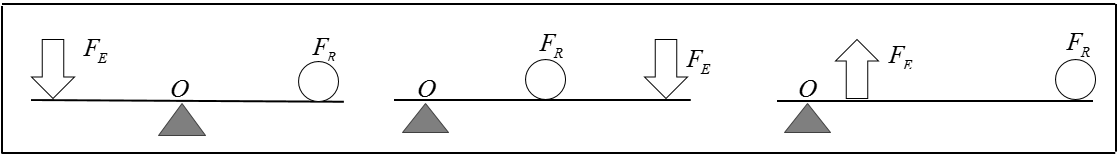
\includegraphics[scale=0.6]{17}
		\end{center}
	\end{enumerate}
	\item {\color{khtug}\sffamily ចូរបំពេញល្បះខាងក្រោមឲ្យបានត្រឹមត្រូវៈ}
	\begin{enumerate}[m]
		\item ឃ្នាស់ដែលមានចំណុចទម្រស្ថិតនៅចន្លោះកម្លាំងចលករ និងកម្លាំងទប់ហៅថា\dotfill។
		\item ផ្ទៃរាបមួយដែលភ្ជាប់ពីកន្លែខ្ពស់ទៅកន្លែងទាបហៅថា\dotfill។
		\item ផលមេកានិចនៃប្រព័ន្ធរ៉កស្មើនឹង\dotfill។
		\item ឃ្នាស់ដែលចល័តជុំវិញអ័ក្សនឹងមួយហៅថា\dotfill។
		\item កម្មន្តឬថាមពលសរុបនៃម៉ាសុីនងាយ =\dotfill+\dotfill។
	\end{enumerate}
	\item {\color{khtug}\sffamily លំហាត់}
	\begin{enumerate}[m]
			\item កម្មករម្នាក់រុញរទះកង់មួយដែលផ្ទុកឥវ៉ាន់ទម្ងន់ $500N$។ ដៃទាំងពីររបស់គាត់ចាប់ត្រង់ចំណុច $A$ ស្ថិតនៅចម្ងាយ $1.45m$ ពីអ័ក្ស $O$ នៃកង់វិល។ សន្មតថាបន្ទុកទាំងអស់ផ្គុំនៅចំណុច $B$ ស្ថិតលើដៃរទះដែលមានចម្ងាយ $0.55m$ ពីអ័ក្សរង្វិលនៃកង់។
			គណនាអាំងតង់សុីតេកម្លាំងដែលកម្មករលើករទះរុញត្រង់ចំណុច $A$។
			\begin{center}
				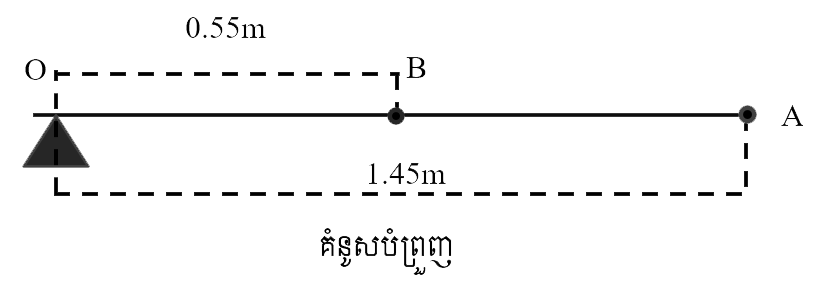
\includegraphics[scale=0.45]{18}
			\end{center}
		\item ជាងជួសជុលរថយន្តម្នាក់ប្រើរ៉កមួយដើម្បីលើកម៉ាសុីនចេញពីរថយន្ត។ម៉ាសុីននោះមានទម្ងន់ $500N$ ហើយត្រូវលើកក្នុងកម្ពស់ $2m$។ ជាងនោះបានប្រើកម្លាំង $200N$ ដើម្បីទាញខ្សែរ៉កចុះក្រោមក្នុងចម្ងាយ $10m$ នៅពេលត្រូវលើក។
		\begin{enumerate}[k]
			\item គណនាកម្មន្តលើកម៉ាសុីន។
			\item គណនាកម្មន្តបំពេញដោយជាង។
			\item គណនាទិន្នផលរបស់រ៉ក។
		\end{enumerate}
	\end{enumerate}
\end{enumerate}
\begin{center}
	\sffamily\color{blue}
	ចប់ជំពូក២
\end{center}
\end{document}